\documentclass[12pt]{article}\usepackage[]{graphicx}\usepackage[]{color}
% maxwidth is the original width if it is less than linewidth
% otherwise use linewidth (to make sure the graphics do not exceed the margin)
\makeatletter
\def\maxwidth{ %
  \ifdim\Gin@nat@width>\linewidth
    \linewidth
  \else
    \Gin@nat@width
  \fi
}
\makeatother

\definecolor{fgcolor}{rgb}{0, 0, 0}
\newcommand{\hlnum}[1]{\textcolor[rgb]{0.69,0.494,0}{#1}}%
\newcommand{\hlstr}[1]{\textcolor[rgb]{0.749,0.012,0.012}{#1}}%
\newcommand{\hlcom}[1]{\textcolor[rgb]{0.514,0.506,0.514}{\textit{#1}}}%
\newcommand{\hlopt}[1]{\textcolor[rgb]{0,0,0}{#1}}%
\newcommand{\hlstd}[1]{\textcolor[rgb]{0,0,0}{#1}}%
\newcommand{\hlkwa}[1]{\textcolor[rgb]{0,0,0}{\textbf{#1}}}%
\newcommand{\hlkwb}[1]{\textcolor[rgb]{0,0.341,0.682}{#1}}%
\newcommand{\hlkwc}[1]{\textcolor[rgb]{0,0,0}{\textbf{#1}}}%
\newcommand{\hlkwd}[1]{\textcolor[rgb]{0.004,0.004,0.506}{#1}}%
\let\hlipl\hlkwb

\usepackage{framed}
\makeatletter
\newenvironment{kframe}{%
 \def\at@end@of@kframe{}%
 \ifinner\ifhmode%
  \def\at@end@of@kframe{\end{minipage}}%
  \begin{minipage}{\columnwidth}%
 \fi\fi%
 \def\FrameCommand##1{\hskip\@totalleftmargin \hskip-\fboxsep
 \colorbox{shadecolor}{##1}\hskip-\fboxsep
     % There is no \\@totalrightmargin, so:
     \hskip-\linewidth \hskip-\@totalleftmargin \hskip\columnwidth}%
 \MakeFramed {\advance\hsize-\width
   \@totalleftmargin\z@ \linewidth\hsize
   \@setminipage}}%
 {\par\unskip\endMakeFramed%
 \at@end@of@kframe}
\makeatother

\definecolor{shadecolor}{rgb}{.97, .97, .97}
\definecolor{messagecolor}{rgb}{0, 0, 0}
\definecolor{warningcolor}{rgb}{1, 0, 1}
\definecolor{errorcolor}{rgb}{1, 0, 0}
\newenvironment{knitrout}{}{} % an empty environment to be redefined in TeX

\usepackage{alltt}


%\usepackage[sans]{../pres1}

\usepackage[hmargin=1in,vmargin=1in]{geometry}
\usepackage{parskip}
%\hypersetup{pdfstartview=FitV,hidelinks}




%% knitr stuff


%% New command for inline code that isn't to be evaluated
\definecolor{inlinecolor}{rgb}{0.878, 0.918, 0.933}         % edit-kwrite
\newcommand{\inr}[1]{\colorbox{inlinecolor}{\texttt{#1}}}
\IfFileExists{upquote.sty}{\usepackage{upquote}}{}
\begin{document}

{
  \Large
  \centering
  {\bf Lab 9 Assignment --- Distance Sampling} \\
  Due before your next lab \par
}

\vspace{10pt}

% Analysis of the (fake) Mongolian gazelle ({\it Procapra gutturosa})
% data using program DISTANCE.  

The purpose of this lab is to learn how to use program DISTANCE or the
R package `Distance' to estimate abundance and density. You will
do this by analyzing fake data on Mongolian gazelle ({\it Procapra
  gutturosa}). The data are fake, but they are based loosely on the
study that we discussed in lecture. Note that gazelles were detected
in groups (ie, herds), and the distance data are distances to group
centers. 

Put your answers in a Word file and upload it to ELC. Name the file
something like ``Chandler-lab9.docx''. Due before your next lab.  




%\clearpage

\section*{Program DISTANCE}

\subsection*{\large Part I: Format data and import into DISTANCE}



\begin{enumerate}
\item Open DISTANCE and create a new project by clicking
  \verb+File > New Project ...+. Name the project something like
  ``Gazelle.dst''  
    
  \item Use the ``New Project Setup Wizard'' and select the
    following options: 
  \begin{enumerate}
    \item Analyze a survey that has been completed
    \item Line transect, single observer, perpendicular distance,
      \textcolor{red}{clusters of objects} 
    \item Distance = Meter, transect length = Kilometers,
      \textcolor{red}{area = Square kilometer}
    \item Do not add any multipliers
    \item \textcolor{red}{Proceed to Data Import Wizard}
  \end{enumerate}


  \item Import Data Wizard
  \begin{enumerate}
    \item Choose the ``GazelleFakeData.txt'' file. %You may need to
 %     select ``All files'' from import window. 
    \item Lowest layer = observation, Highest layer = region. Accept
      other defaults on Step 3 window and then hit ``Next''. 
    \item On next window, tell it to ignore first row of data by
      checking the box labeled `Do not import first row'. Hit Next. 
    \item On the ``Step 5'' window, you need to label columns
      (``layer'') by clicking on the grey boxes above each column. 
      \begin{itemize}
        \item[(i)] Label the Transect column as: line transect, label,
          label  
        \item[(ii)] Tell it to ignore the GroupID column
        \item[(iii)] Label distance column as: observation, perpendicular
          distance, decimal 
        \item[(iv)] Label the group size column as: observation, cluster
          size, decimal 
        \item[(v)] Label transect length column as: line transect, line
          length, decimal 
        \item[(vi)] Label area column as: region, area, decimal
      \end{itemize}
    \item Hit Next, and then choose ``Overwrite existing data''. 
  \end{enumerate}
  \item Hit Next again, and then click on ``Observation'' on the left to
    display the data. You should see data like that shown in Fig. 1
    below. Area refers to the area covered by the 10 transects,
    which were 100 km long and 250 m wide. Cluster size is the number
    of gazelle detected in each group. 
\end{enumerate}

\begin{figure}[h!]
  \centering
  \fbox{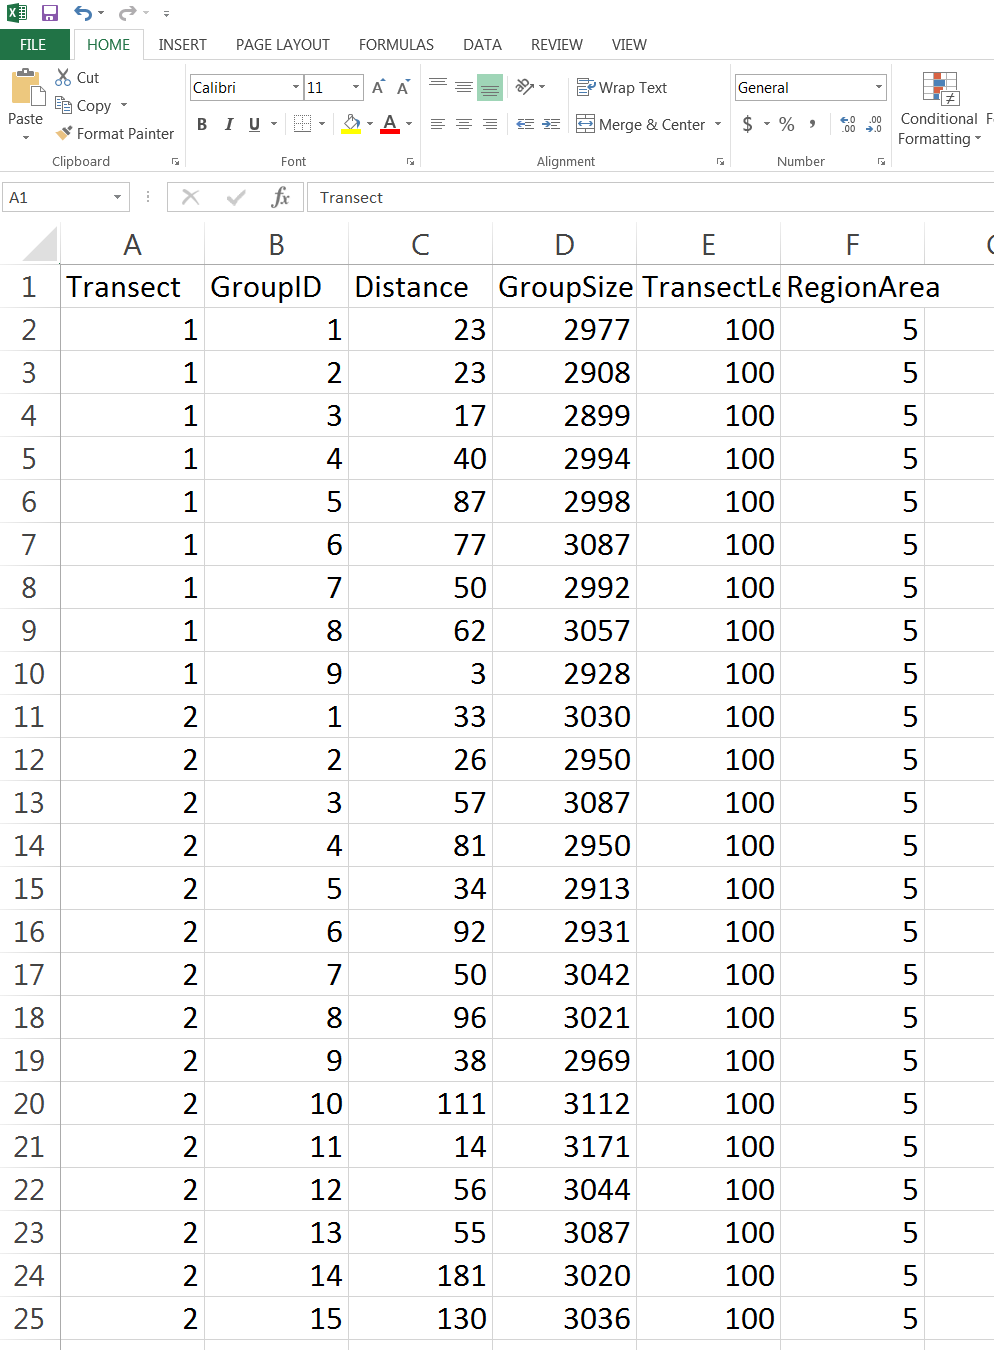
\includegraphics[height=8.5cm]{figs/ds-data1}} \hfill
  \fbox{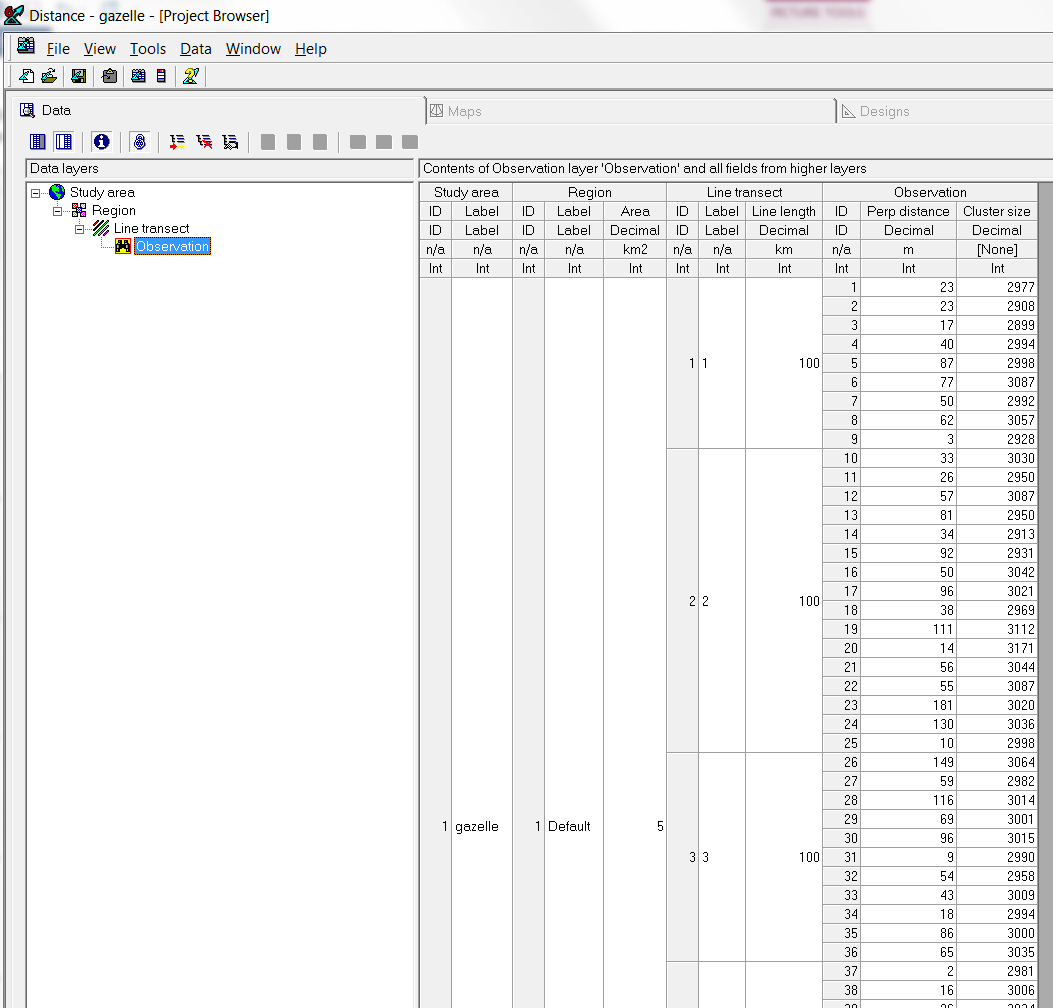
\includegraphics[height=8.5cm]{figs/ds-data2}}   \\
  \caption{\small Data formatted in Excel (left) and the same data in
    program DISTANCE.} 
  \label{fig:ds-data}
\end{figure}
%\clearpage



\clearpage

\subsection*{\large  Part II -- Estimate gazelle density and abundance}

\subsubsection*{\normalsize Half-normal detection function}


\begin{enumerate}
  \item Click the ``Analyses'' tab, then right click on the ``New 
    analysis'' line, and then choose ``Analysis details''.  
  \item Name this analysis ``Half-normal''
  \item Under ``data filters'', click on ``Properties'' and
    name the data filter ``truncate250''. Click on the ``Truncation''
    tab and tell it to discard all observations beyond 250m. Hit
    OK. 
  \item Under ``model definitions'' choose ``Properties'' and
    name it ``HN'' for half-normal. Then click the ``Detection
    function'' tab. Under ``Models'', specify a model with a
    half-normal ``key function''. Next, click on ``Adjustment terms''
    and choose ``Manual selection'' with 0 adjustment terms. Click the
    ``Cluster size'' tab and choose ``Use mean of observed
    clusters''. Hit ``OK''. 
  \item Run the model.
  \item On the ``Results'' tab on the right, scroll through the
    pages to the histograms of detection distances and the fitted
    detection function. Find the one that looks the best, in terms of
    the detection function fitting the histogram well, and then copy
    and paste it into your Word file. The easiest way to do this is to
    copy and paste into MS Paint and then save it as an image
    file. Then use \verb+Insert > Picture+ in Word.  Or you can take a
    screen shot of the histogram and paste that in. 
  \item Add a figure caption below the histogram that explains
    the graph.   
  \item Create a table to report estimates of abundance (N), density
    (D), group density (DS), sigma (called A(1) in DISTANCE), and
    p. Include standard errors (SEs) and confidence intervals (CIs) in
    your table. Define each of the parameters in your table (one sentence per parameter). 
\end{enumerate}


\subsubsection*{\normalsize Hazard-rate detection function}

\begin{enumerate}
  \item Run a second analysis in which you use a ``hazard-rate''
    detection function instead of the half-normal detection
    function. Do this by closing the results window, and
    right-clicking under the ``Analyses'' tab to select ``New Analysis\dots''.  
  \item Next, right-click on the new line that appeared (should be
    highlighted in blue) and choose `Analysis Details' again as you
    did before. Change the name of the analysis, and create a new
    `Model definition' in which you change the key function to
    `hazard-rate'. For all other options, use the same settings as
    before.   
  \item Repeat steps 6-7 above. Why do you think the results differ
    when you use different detection functions? Which of the two
    models is better (has the lower AIC)?  
\end{enumerate}


\clearpage


\section*{R package `Distance'}

Open R (or RStudio) and install the package using the following
command: 

\begin{knitrout}
\definecolor{shadecolor}{rgb}{0.878, 0.918, 0.933}\color{fgcolor}\begin{kframe}
\begin{alltt}
\hlkwd{install.packages}\hlstd{(}\hlstr{"Distance"}\hlstd{)}
\end{alltt}
\end{kframe}
\end{knitrout}

Several other packages will be installed during the process. Now we
can load the package like so: 

\begin{knitrout}
\definecolor{shadecolor}{rgb}{0.878, 0.918, 0.933}\color{fgcolor}\begin{kframe}
\begin{alltt}
\hlkwd{library}\hlstd{(Distance)}
\end{alltt}


{\ttfamily\noindent\itshape\color{messagecolor}{\#\# Loading required package: mrds}}

{\ttfamily\noindent\itshape\color{messagecolor}{\#\# This is mrds 2.2.3\\\#\# Built: R 4.0.3; ; 2020-10-17 13:10:23 UTC; unix}}

{\ttfamily\noindent\itshape\color{messagecolor}{\#\# \\\#\# Attaching package: 'Distance'}}

{\ttfamily\noindent\itshape\color{messagecolor}{\#\# The following object is masked from 'package:mrds':\\\#\# \\\#\#\ \ \ \  create.bins}}\end{kframe}
\end{knitrout}

Before we can do any analysis, we need to import the Mongolian gazelle
data. Make sure that the file \texttt{GazelleFakeData.txt} is in your
working directory.

\begin{knitrout}
\definecolor{shadecolor}{rgb}{0.878, 0.918, 0.933}\color{fgcolor}\begin{kframe}
\begin{alltt}
\hlkwd{getwd}\hlstd{()}       \hlcom{## Location on your computer where R will look for files}
\end{alltt}
\begin{verbatim}
## [1] "/home/rchandler/courses/applied-popdy/labs/distance"
\end{verbatim}
\begin{alltt}
\hlkwd{list.files}\hlstd{()}  \hlcom{## You should see 'GazelleFakeData.txt' here}
\end{alltt}
\begin{verbatim}
## [1] "auto"                "figs"                "GazelleFakeData.txt"
## [4] "lab-distance.pdf"    "lab-distance.Rnw"    "lab-distance.tex"
\end{verbatim}
\end{kframe}
\end{knitrout}

If you need to change your working directory, you can use the dropdown
menu options, or you can use a command like this:

\begin{knitrout}
\definecolor{shadecolor}{rgb}{0.878, 0.918, 0.933}\color{fgcolor}\begin{kframe}
\begin{alltt}
\hlkwd{setwd}\hlstd{(}\hlstr{"C:/Users/RichardC/courses/"}\hlstd{)} \hlcom{## Change the path in quotes!}
\end{alltt}
\end{kframe}
\end{knitrout}

Once you have the data file in your working directory, you can import
the fake gazelle data. The data file is a tab-separated text file
instead of a comma-seperated text file like we used last week:

\begin{knitrout}
\definecolor{shadecolor}{rgb}{0.878, 0.918, 0.933}\color{fgcolor}\begin{kframe}
\begin{alltt}
\hlstd{gazelleData} \hlkwb{<-} \hlkwd{read.table}\hlstd{(}\hlstr{"GazelleFakeData.txt"}\hlstd{,} \hlkwc{header}\hlstd{=}\hlnum{TRUE}\hlstd{,} \hlkwc{sep}\hlstd{=}\hlstr{"\textbackslash{}t"}\hlstd{)}
\end{alltt}
\end{kframe}
\end{knitrout}

The structure of the data can be assessed like this:

\begin{knitrout}
\definecolor{shadecolor}{rgb}{0.878, 0.918, 0.933}\color{fgcolor}\begin{kframe}
\begin{alltt}
\hlkwd{str}\hlstd{(gazelleData)}
\end{alltt}
\begin{verbatim}
## 'data.frame':	118 obs. of  6 variables:
##  $ Transect      : int  1 1 1 1 1 1 1 1 1 2 ...
##  $ GroupID       : int  1 2 3 4 5 6 7 8 9 1 ...
##  $ Distance      : int  23 23 17 40 87 77 50 62 3 33 ...
##  $ GroupSize     : int  2977 2908 2899 2994 2998 3087 2992 3057 2928 3030 ...
##  $ TransectLength: int  100 100 100 100 100 100 100 100 100 100 ...
##  $ RegionArea    : int  5 5 5 5 5 5 5 5 5 5 ...
\end{verbatim}
\end{kframe}
\end{knitrout}

We have to reformat the data to meet the requirements of the Distance
package. The code below creates a new data frame, renames the columns,
and converts the distance units to kilometers.

\begin{knitrout}
\definecolor{shadecolor}{rgb}{0.878, 0.918, 0.933}\color{fgcolor}\begin{kframe}
\begin{alltt}
\hlstd{gazelleData2} \hlkwb{<-} \hlstd{gazelleData[,}\hlkwd{c}\hlstd{(}\hlstr{"Transect"}\hlstd{,} \hlstr{"GroupSize"}\hlstd{)]}
\hlkwd{colnames}\hlstd{(gazelleData2)} \hlkwb{<-} \hlkwd{c}\hlstd{(}\hlstr{"Sample.Label"}\hlstd{,} \hlstr{"size"}\hlstd{)}
\hlstd{gazelleData2}\hlopt{$}\hlstd{distance} \hlkwb{<-} \hlstd{gazelleData}\hlopt{$}\hlstd{Distance} \hlopt{/} \hlnum{1000} \hlcom{## Convert to km}
\hlstd{gazelleData2}\hlopt{$}\hlstd{Region.Label} \hlkwb{<-} \hlnum{1}
\hlstd{gazelleData2}\hlopt{$}\hlstd{Effort} \hlkwb{<-} \hlstd{gazelleData}\hlopt{$}\hlstd{TransectLength}
\hlstd{gazelleData2}\hlopt{$}\hlstd{Area} \hlkwb{<-} \hlstd{gazelleData}\hlopt{$}\hlstd{RegionArea}
\end{alltt}
\end{kframe}
\end{knitrout}

The distance sampling model can be fitted to the data using the
\inr{ds} function. The \inr{key} argument specifies the detection
function. You could switch from the half-normal to the hazard-rate
function using: \inr{key="hr"}.


\begin{knitrout}
\definecolor{shadecolor}{rgb}{0.878, 0.918, 0.933}\color{fgcolor}\begin{kframe}
\begin{alltt}
\hlstd{model.hn} \hlkwb{<-} \hlkwd{ds}\hlstd{(}\hlkwc{data}\hlstd{=gazelleData2,} \hlkwc{key}\hlstd{=}\hlstr{"hn"}\hlstd{,}
               \hlkwc{transect}\hlstd{=}\hlstr{"line"}\hlstd{,} \hlkwc{truncation}\hlstd{=}\hlnum{250}\hlopt{/}\hlnum{1000}\hlstd{,}
               \hlkwc{adjustment}\hlstd{=}\hlkwa{NULL}\hlstd{,} \hlkwc{quiet}\hlstd{=}\hlnum{TRUE}\hlstd{)}
\end{alltt}


{\ttfamily\noindent\itshape\color{messagecolor}{\#\# Fitting half-normal key function}}

{\ttfamily\noindent\itshape\color{messagecolor}{\#\# Key only model: not constraining for monotonicity.}}

{\ttfamily\noindent\itshape\color{messagecolor}{\#\# AIC= -430.39}}\end{kframe}
\end{knitrout}

Once you have fitted the model, you can obtain the parameter estimates
using the following command:

\begin{knitrout}
\definecolor{shadecolor}{rgb}{0.878, 0.918, 0.933}\color{fgcolor}\begin{kframe}
\begin{alltt}
\hlkwd{summary}\hlstd{(model.hn)}
\end{alltt}
\end{kframe}
\end{knitrout}

To view the estimated detection function, do this:

\begin{knitrout}
\definecolor{shadecolor}{rgb}{0.878, 0.918, 0.933}\color{fgcolor}\begin{kframe}
\begin{alltt}
\hlkwd{plot}\hlstd{(model.hn)}
\end{alltt}
\end{kframe}
\end{knitrout}


Answer all of the questions listed under ``Part II'' above.


\end{document}




